\section{Observations and Opportunities} 
\label{sec:observations}

In this section, we characterize the performance-energy behavior of LLaMA-3.1-8B~\cite{grattafiori2024llama} served by SGLang~\cite{zheng2024sglang} on an A100 GPU.
We profile key metrics, including TTFT, ITL, and end-to-end (E2E) energy consumption (measured via NVIDIA Management Library~\cite{nvml}).
Furthermore, we analyze real-world workload traces, the Azure LLM Inference Trace 2024 dataset~\cite{stojkovic2025dynamollm}, to identify temporal and batching patterns.

\begin{figure}[t]
    \centering
    \begin{subfigure}[b]{0.49\columnwidth}
        \centering
        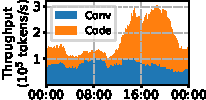
\includegraphics[width=\linewidth]{figs/TPS_IN.pdf}
        \caption{Prefill throughput.}
        \label{fig:pd-ratio-prefill}
    \end{subfigure}
    \hfill
    \begin{subfigure}[b]{0.49\columnwidth}
        \centering
        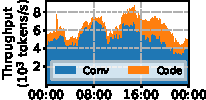
\includegraphics[width=\linewidth]{figs/TPS_OUT.pdf}
        \caption{Decode throughput.}
        \label{fig:pd-ratio-decoding}
    \end{subfigure}
    % \begin{subfigure}[b]{\columnwidth}
    %     \centering
    %     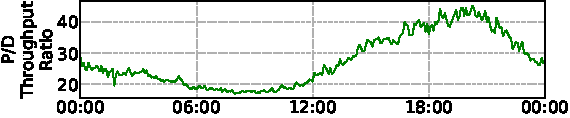
\includegraphics[width=\linewidth]{figs/ratio.pdf}
    %     \caption{P/D throughput ratio (code + conversation) in a weekday.}
    %     \label{fig:pd-ratio-in-a-day}
    % \end{subfigure}
    \caption{Temporal variations of prefill and decode throughput in Azure LLM Inference Trace 2024 dataset. Conversation and code requests exhibit distinct diurnal patterns. Colors are stacked.}
    \label{fig:pd-ratio}
\end{figure}

\subsection{Multi-Timescale Workload Dynamics in LLM Serving}
% Temporal Variation in Prefill-Decode Demand and Iteration-Level Workload Fluctuations}
\label{subsec:temporal-variation}

% \jiahuan{@Minjia, I suggest to remove this part as we discussed in the slack channel}
% \minjia{I restructured and revised the section. Please take a look.}
% \jiahuan{My thought is, in this subsection, we should explain two things: \begin{enumerate}
%     \item why we use the P/D disaggregation architecture.
%     \item why per-iteration frequency responsiveness is important.
% \end{enumerate}
% In current version, we explain them by: \begin{enumerate}
%     \item varying P/D demands in real world trace
%     \item as \fref{fig:prefill-tokens-fluctuation} shows, there are significant workload fluctuation between convective iterations in the prefill instance.
% \end{enumerate}
% However, there are potential logic problems: \begin{enumerate}
%     \item assuming we have per-iteration frequency responsiveness, for P/D collocated architecture, we can set different frequency for each prefill or decode batch. Reviewers may think we don't really need a P/D disaggregated architecture to mitigate the P/D demand variation.
%     \item as we discussed before, if we mention the Azure LLM inference dataset here, we'd better add a small section in analysis to show the result on such real-world trace.
% \end{enumerate}
% I believe we have another option to write this subsection:\begin{enumerate}
%     \item For P/D collocated architecture, there are interference between the prefill and the decode phases, as \fref{fig:pd-collocated} shows. Suppose the decode iteration consumes 20ms, and the prefill (or P/D mixed if chunked prefill is enabled) iteration consumes 300ms: \begin{itemize}
%         \item if chunked prefill is OFF: if there's prefill iteration between two decode iterations, the inference time of the prefill iteration contributes to the ITL. Considering prefill inference time is usually significantly longer than ITL SLO, in most cases, even at the highest frequency, it still leads to ITL SLO violations. Thus, we have no opportunities to lower down the GPU frequency during the decode iterations.
%         \item if chunked prefill is ON: some ITLs come from P+D mixed iteration. Due to the typically longer time of P+D mixed iteration than the ITL SLO, we must set it to highest frequency, just as the prefill iteration in the case where chunked prefill is OFF.
%     \end{itemize}
%     For P/D disaggregated architecture, there're no such issues. ITL mainly comes from the inference time of decode iterations. Thus we can employ the frequency adjustment for the decode iterations.
% \end{enumerate}
% In \sref{subsec:pd-dist} you mention the ``Systems such as SplitWise~\cite{patel2024splitwiseefficientgenerativellm}, TetriInfer~\cite{tetrinfer}, Llumnix ~\cite{llumnix} and DistServe~\cite{zhong2024distserve} show that this separation improves goodput and TTFT and ITL SLO attainment rate  by avoiding phase-level contention and enabling distinct execution policies.''
% \fref{fig:pd-collocated} actually provides the examples of the ``phase-level contention'', and why it creates the obstacle for energy efficient LLM serving.
% \begin{figure}
%     \centering
%     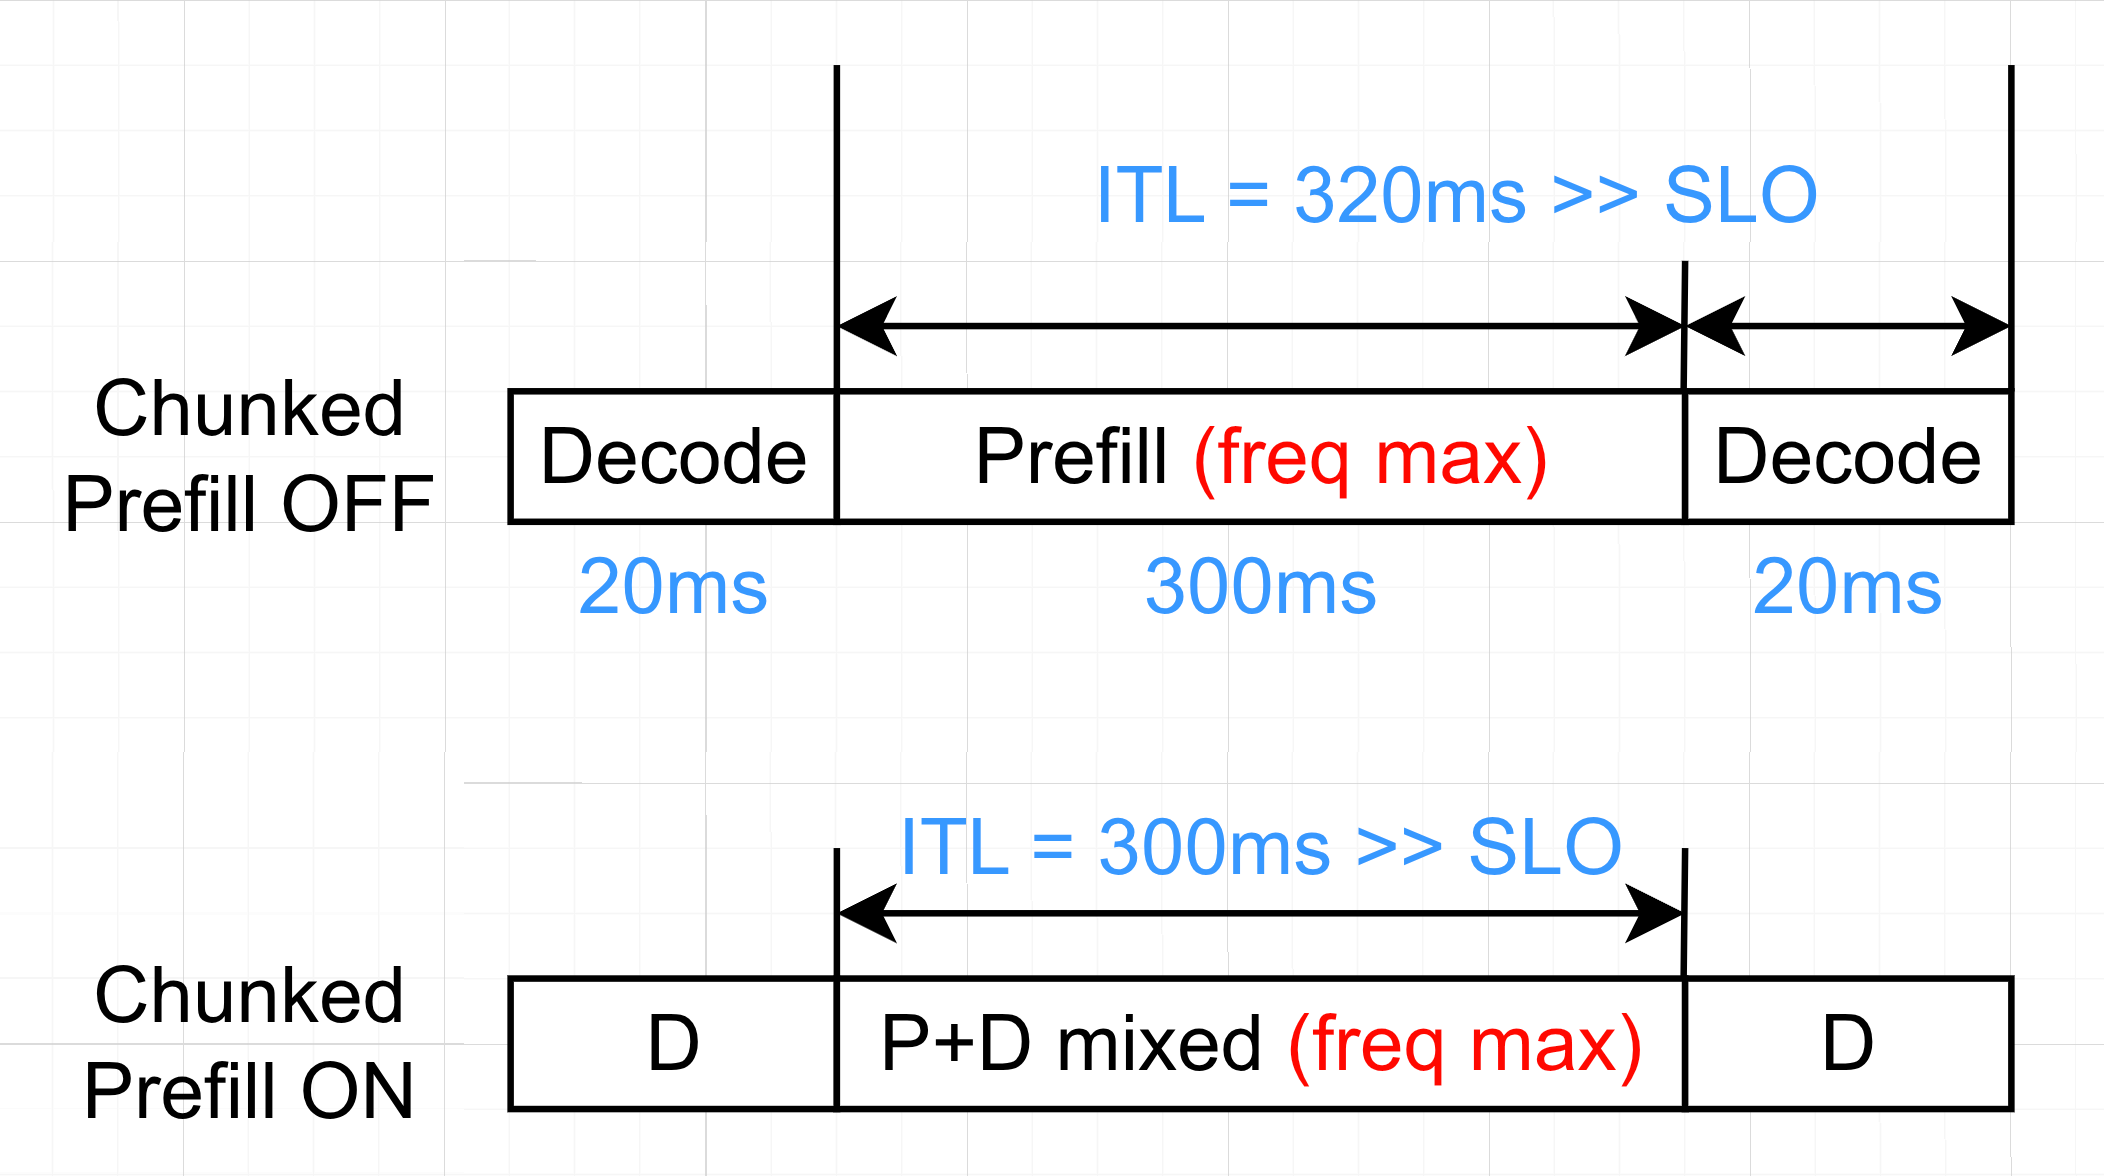
\includegraphics[width=\columnwidth]{figs/GetImage.png}
%     \caption{P/D interference on the collocated architecture.}
%     \label{fig:pd-collocated}
% \end{figure}
% \minjia{Good thoughts. Agreed to the "should explain two things". For why we use P/D disaggregation, I had an implicit assumption that in order to meet both TTFT/TBT SLO requirements in coupled architecture, it is extremely hard to set a single frequency (even per-iteration) without violating TTFT/TBT SLOs. It feels that this is intuitive, because having controlled TTFT/TBT SLO control is exactly one of the main motivation behind P/D-dist. Therefore, if we tackle SLO-aware energy-efficient LLM inference, we inherit the benefits of SLO-awareness from P/D-dist. Based on my understanding of your write-up, you are trying to back up this claim with evidence to better motivate why choosing P/D-dist architecture, right? }}
% \jiahuan{right. If we only talk about the P/D ratio variation, some reviewers who are not very familiar with P/D disaggregation may ask ``assuming we have per-iteration frequency responsiveness, for P/D collocated architecture, we can set different frequency for each prefill or decode batch. Reviewers may think we don't really need a P/D disaggregated architecture to mitigate the P/D demand variation.''}
% \jiahuan{you say ``It feels that this is intuitive''. But I'm not sure it is really intuitive for the reviewers. Maybe we can use few sentences to give more details? about the P/D interference in collocated architecture}
% \minjia{Got it. It could raise issues. My thinking for this first observation: (i) establish that energy adaptation is possible (workload variation), and (ii) fine-grained energy adaptation is also possible but hard to achieve (high fluctuation). Both of these motivate our approach (energy control). Adding additional results to justify why using P/D is helpful but it does not lead to any real technical contribution (simply choosing PD disaggregation cannot be a technical contribution although we can claim we are the first to have SLO-aware energy control on disaggregated LLM inference). Let's first try to address this by adding a few sentences to see if we can convincingly deliver why collocated architecture may not be a good choice for handling P/D demand variation while satisfying SLO guarantees? But overall, it feels that to the current observation I at least helps deliver (i) and (ii) above.}
% \jiahuan{sounds good. agree that (i) (ii) are clearly delivered. I'll try to add some additional sentences to talk the third point.}
% \minjia{Right. If we have time and space and would like to make the logic chain stronger, then totally agreed that what you propose can strengthen the paper.}
% \jiahuan{sounds good. I'm revising the observation section. Please look at system design section C D E if you are available}
% \minjia{One potential result to show that may help motivate P/D: By setting a lower frequency, the SLO attainment rate drops noticeably for both TTFT/TBT. This motivate workload-aware frequency control.}
% \minjia{I have a proposal deadline today and a talk tomorrow. It is also ICLR rebuttal period. I will try to read more tomorrow afternoon and during the weekend.}
% \jiahuan{ok, take your time.}
% \minjia{One suggestion: kindly collect the items mentioned in the ASPLOS reviews and add one phrase to indicate if we have addressed it somehow. }
% \jiahuan{I will do that}

% Real-world LLM workloads exhibits significant temporal variation across both request types and phases.
% We analyze the Azure LLM Inference Trace 2024 dataset, which contains requests sampled from LLM inference services in Microsoft Azure.
% The dataset categorizes requests into two types: \textit{conversation} and \textit{code}.
% As shown in \fref{fig:pd-ratio-prefill}, the prefill throughput of conversation requests remains relatively stable in a day, while code requests exhibit a significant diurnal pattern, peaking in the afternoon and evening.
% Furthermore, code requests typically have shorter decode lengths.
% Consequently, as depicted in \fref{fig:pd-ratio-decoding}, the overall variation of the decode throughput is much smaller than prefill.
% For a system handling both request types concurrently, this shifting workload composition leads to significant variation in the overall P/D throughput ratio throughout the day, as shown in \fref{fig:pd-ratio-in-a-day}.

% This dynamic workload pattern variation presents both a significant challenge and a unique opportunity for energy efficiency.
% On one hand, a unified frequency scaling strategy is problematic: optimizing GPU frequency solely for one phase can degrade the performance of the other.
% On the other hand, this pattern allows aggressive energy savings if independently scaling frequency for the two phases, outperforming the policy that treats them uniformly.
% The P/D disaggregated architecture for LLM serving perfectly matches this independent control policy.


% \jiahuan{TODO: \appref{subsubsec:pd-interference}}

Real-world LLM workloads exhibit variation at two distinct timescales.
At a \emph{coarse-grained} level, request arrival rates and prompt lengths fluctuate significantly over time, leading to shifting prefill-decode throughput demand and motivating energy adaptation.
Taking the Azure LLM Inference Trace 2024 dataset~\cite{stojkovic2025dynamollm} as an example, it categorizes requests into two types: \emph{conversation} and \emph{code}.
As shown in \fref{fig:pd-ratio-prefill}, the prefill throughput of conversation requests remains relatively stable over a day, while code requests exhibit a significant diurnal pattern, peaking in the afternoon and evening.
Furthermore, code requests typically have shorter decode lengths.
Consequently, as depicted in \fref{fig:pd-ratio-decoding}, the overall variation of the decode throughput is much smaller than that of prefill.
At a \emph{fine-grained} level, the number of active tokens and requests in prefill changes rapidly over time, as shown in \fref{fig:prefill-tokens-fluctuation}, due to dynamic batching, request completion, and various request lengths, which create short-term load fluctuations that directly affect GPU utilization and latency.
These P/D demand variations motivate phase-specific and workload-aware energy adaptation.
Most importantly, these fast dynamics also make static or coarse adjustments ineffective, highlighting the need for more responsive frequency control for energy efficiency. 



\textbf{\underline{Insight \#1}}:
Real-world LLM inference workloads vary across two timescales: coarse-grained shifts in prefill-decode demand and fine-grained, iteration-level fluctuations in prefill batch composition.
These multi-timescale dynamics make static or coarse frequency control policies ineffective, motivating a phase-specific and responsive approach for energy-efficient LLM serving with SLO guarantees. 



% \begin{figure}[!ht]
%     \centering
%     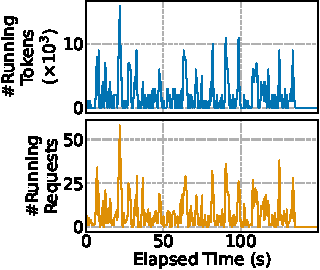
\includegraphics[width=\columnwidth]{figs/prefill-load-bs-time.pdf}
%     \caption{Rapid iteration-level workload fluctuations in the number of running requests and running tokens of the prefill phase.}
%     % It leads to highly dynamic instantaneous load, which motivates responsive, iteration-level frequency control.}
%     \jiahuan{@junfeng, Stack this figure vertically. fix the y aixs label for the left figure and y axis label for the right figure}
%     \label{fig:prefill-tokens-fluctuation}
% \end{figure}

\begin{figure}[!t]
    \centering
    \begin{minipage}[b]{0.49\columnwidth}
        \centering
        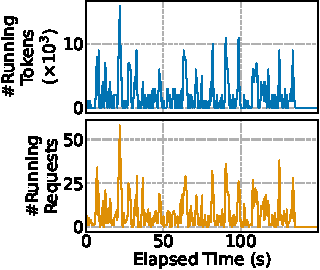
\includegraphics[width=\columnwidth]{figs/prefill-load-bs-time.pdf}
        \caption{Rapid iteration-level workload fluctuations of running requests and  tokens of the prefill phase.}
        % \jiahuan{@Junfeng, squeeze height: can use 3 lines for y-axis label, ``Reqs'' $\to$ Requests}
        % It leads to highly dynamic instantaneous load, which motivates responsive, iteration-level frequency control.}
        \label{fig:prefill-tokens-fluctuation}
    \end{minipage}
    \hfill
    \begin{minipage}[b]{0.49\columnwidth}
        \centering
        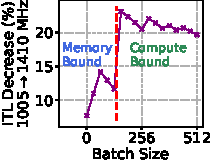
\includegraphics[width=\linewidth]{figs/decode_itl_diff.pdf}
        \caption{Decode ITL decrease percentage from frequency scaling (1005 $\to$ 1410 MHz) under various batch sizes.}
        % \jiahuan{may merge with \fref{fig:prefill-tokens-fluctuation} if space is the problem}
        \label{fig:decode-itl-diff}
        % \jiahuan{TODO: redraw it to adjust height}
    \end{minipage}
\end{figure}

\subsection{U-Shaped Energy-Frequency Relationship and Sensitivities in P/D Disaggregated LLM Serving} \label{sec:obs-u-shape}

% Our analysis in \sref{sec:intro} reveals a U-shaped energy-frequency curve for LLM inference, implying the existence of an energy-efficiency sweet spot.
% We extend this analysis to a P/D disaggregated architecture.
% Both phases independently exhibit this U-shaped relationships, but their characteristics differ due to distinct workload and compute/memory access characteristics.

Frequency scaling is a common technique for energy optimization, yet its effect on LLM inference is non-monotonic.
Our measurements in \fref{fig:u-shape-coupled} reveal a clear U-shaped energy-frequency relationship, which indicates an energy-efficiency sweet spot.
To understand how this behavior manifests under P/D disaggregation, we  examine the two phases separately.

\fref{fig:u-shape} shows the energy and latency characteristics of the two phases across various GPU frequencies, using requests with varied input and output lengths for each phase.
% and input/output request lengths for each phase.
Both phases show monotonically decreasing latency-frequency curves and U-shaped energy-frequency curves, with 1005 MHz consistently being the energy-optimal point before a sharp energy upsurge towards the maximum frequency (1410 MHz).
Frequencies below 1005 MHz are strictly suboptimal, as they increase both energy and latency.
However, the two phases differ markedly in shape and sensitivity, stemming from fundamental architectural factors.

According to~\cite{gonzalez1997supply}, the power $P$ of CMOS circuits (i.e., the physical foundation of GPUs) comprises a frequency-irrelevant static part and a frequency-dependent dynamic part:
\begin{equation}
    P = P_{\textbf{static}} + P_{\textbf{dynamic}} \approx P_{\textbf{static}} + CV^2f \sim A + B f^{1+\alpha},
\end{equation}
where $A$, $B$, $C$, $\alpha$ are coefficients, $V$ is voltage, which also increases with frequency.
We denote this change as $V^2\sim f^\alpha$, where $\alpha>0$ and can increase with $f$.
Thus, the execution time $T$ and energy consumption $E$ can be expressed as:
\begin{align}
    T &\sim f^{-\beta} \sim \left[(P-A)/B\right]^{-\beta/(1+\alpha)}, \label{eq:t-alpha-beta} \\
    E &= PT \sim A f^{-\beta} + B f^{1+\alpha - \beta}, \label{eq:u-shape} 
\end{align}
where $0\le\beta\le1$ is an arithmetic intensity-related coefficient: 
$\beta=1$ indicates fully compute-bound, and $\beta=0$ indicates fully memory-bound.
The $E$-$f$ plot of \eref{eq:u-shape} is a U-shaped curve, as the $A f^{-\beta}$ term dominates at low frequencies and the $B f^{1+\alpha - \beta}$ term dominates at high frequencies.
This theoretical analysis matches our empirical observation in \fref{fig:u-shape}.
Furthermore, for the compute-bound prefill phase, $\beta\approx1$, which means it benefits almost proportionally from higher frequency (\eref{eq:t-alpha-beta}) and gets significant TTFT reduction at the cost of higher energy (\fref{fig:u-shape-p} bottom), quickly driving the GPU toward its Thermal Design Power (TDP) limit at $\approx$1305 MHz.
In contrast, for the common memory-bound decode phase, $\beta<1$, which means decode derives a sub-linear benefit from higher frequency (\eref{eq:t-alpha-beta}), as \fref{fig:u-shape-d} bottom shows:  increasing $f$ from 1005 MHz to 1410 MHz yields only $\approx$20\% ITL reduction at the cost of $\approx$50\% higher energy.
Notably, as batch size grows and arithmetic intensity increases, decode gradually transitions toward compute-bound behavior and responds more strongly to higher frequencies (\fref{fig:decode-itl-diff}). 

% where $0\le\beta\le1$ is atrithmetci intensiy realted coeffcient.
% For idea conput bound senaroi, $\beta=0$, for total memory bound, $\beta=1$.
% The plot of \eref{eq:u-shape} is a U-shaped curve, as the first term ($A f^{\beta-1}$) dominates at low frequencies (time-dominated) and the second term ($B f^{\alpha + \beta}$) dominates at high frequencies (power-dominated).
% This theoretical model matches our empirical observation in \fref{fig:u-shape}.
% Furthermore, for the compute bound prefill, $\beta\approx0$, means it can get alopmst all benefit from higher frequency, just as \fref{fig:u-shape-p} bottom shows, quickly driving the GPU toward its Thermal Design Power (TDP) limit at $\approx$1305 MHz.
% While for the common memeory-bound decode, $\beta>1$, it means decode get sub -linearly benefit from higher frequency, just as \fref{fig:u-shape-d} bottom, i.e., increasing frequency from 1005 MHz to 1410 MHz yields only $\approx$20\% ITL reduction at the cost of $\approx$50\% higher energy.



% According to~\cite{gonzalez1997supply}, the dynamic power $P$ of CMOS circuits (the physical foundation of GPU) increases hyper-linearly with frequency $f$ when $f$ is high, due to increased voltage $V$.
% This is commonly modeled as:
% \begin{equation}
%     P \propto V^2f \propto f^{1+\alpha}\ (\alpha > 0, \text{when}\ f\ \text{is high}). \label{eq:P-f}
% \end{equation}
% Prefill is compute-bound, and quickly drives the GPU toward its Thermal Design Power (TDP) limit at $\approx$1305 MHz.
% Its execution time therefore scales roughly inversely with frequency:
% \begin{equation}
%     T_{\text{prefill}} \propto f^{-1}   \propto P^{-\frac{1}{1+\alpha}}, \label{eq:prefill-f} 
% \end{equation}
% yielding significant TTFT reductions that scale more proportional to the energy cost (as \fref{fig:u-shape-p} bottom shows).
% Decode, in contrast, remains below the TDP limit for typical batch sizes and is largely memory-bound, so its execution time improves only sub-linearly with frequency:
% \begin{equation}
%     T_{\text{decode}} \propto f^{-(1-\beta)}  \propto P^{-\frac{1-\beta}{1+\alpha}}\ (0<\beta<1). \label{eq:decode-f}
% \end{equation}
% As a result, \fref{fig:u-shape-d} bottom shows that increasing frequency from 1005 MHz to 1410 MHz yields only $\approx$20\% ITL reduction at the cost of $\approx$50\% higher energy.
% Furthermore, as batch size grows and arithmetic intensity increases, decode gradually transitions toward compute-bound behavior and responds more strongly to higher frequencies (\fref{fig:decode-itl-diff}). 
% Together, these effects explain the distinct U-shape energy-frequency curves in P/D phases and motivate phase-specific energy control strategies. 





% \jiahuan{revise it after updating figure}


% As batch size grows and arithmetic intensity increases (\fref{fig:decode-itl-diff}), decode gradually transitions toward compute-bound behavior and responds more strongly to higher frequencies. Together, these effects explain the distinct U-shape energy-frequency curves in prefill and decode and motivate phase-specific energy control strategies. 


% TDP-limited near 1305 MHz, whereas decode is often memory-bound and yields only $\approx$20\% ITL reduction for $\approx$50\% higher energy when increasing frequency from 1005 to 1410 MHz.}
    % These phase-specific trade-offs motivate independent and adaptive frequency control.


% As a result, increasing the frequency from 1005 MHz to 1410 MHz yields only $\approx$20\% ITL reductions at the cost of $\approx$50\% higher energy, whereas prefill gains more proportional TTFT reductions from higher frequencies.

% As batch size grows and arithmetic intensity increases (\fref{fig:decode-itl-diff}), decode gradually transitions toward compute-bound behavior and responds more strongly to higher frequencies. Together, these effects explain the distinct U-shape energy-frequency curves in prefill and decode and motivate phase-specific energy control strategies. 

% Prefill is compute and power-intensive, hitting the GPU's Thermal Design Power (TDP) limit at $\sim$1305 MHz.
% Decode remains below the TDP limit but shows sub-linear latency gains: increasing frequency from 1005 MHz to 1410 MHz yields only $\approx$20\% ITL reductions at the cost of $\approx$50\% higher energy, whereas prefill gains more proportional TTFT reductions from higher frequencies.
% \fref{fig:decode-itl-diff} further shows that as the batch size increases, the decode phase gradually transitions from memory-bound to compute-bound, thus the ITL benefits from frequency scaling become more pronounced.

% \jiahuan{TODO: may move to appendix if the space is the problem}
% \jiahuan{@Minjia, should we move this to the system design section? As it seems too involved}
% \minjia{Yes. Temporarily move it to here.}
% The U-shaped curve and P/D phase differences can be explained by two underlying factors.
% These contrasting behaviors stem from fundamental architectural factors.
% % First, the dynamic power $P$ of CMOS circuits increases hyper-linearly with GPU frequency $f$ due to voltage $V$ scaling~\cite{gonzalez1997supply}, commonly modeled as:
% % (\eref{eq:P-f}).
% % \begin{align}
% %     P & \propto V^2f \propto f^{1+\alpha}\ (\alpha > 0, \text{when}\ f\ \text{is high}) \label{eq:P-f}
% % \end{align}
% Prefill is compute-bound, and quickly drives the GPU toward its Thermal Design Power (TDP) limit at around 1305 MHz. Its execution time therefore scales roughly inversely with frequency, 
% \begin{align}
%     T_{\text{prefill}} & \propto f^{-1}   \propto P^{\frac{1}{1+\alpha}} \label{eq:prefill-f} 
% \end{align}
% yielding strong TTFT reductions but rapidly increasing energy as the dynamic power $P$ of CMOS circuits increases hyper-linearly with GPU frequency $ P \propto V^2f \propto f^{1+\alpha}\ (\alpha > 0, \text{when}\ f\ \text{is high})$~\cite{gonzalez1997supply}. 
% Decode, in contrast, remains well below the TDP limit for typical batch sizes and is largely memory-bound, so its execution time improves only sublinearly with frequency,
% \jiahuan{add reference}
% \begin{align}
%     T_{\text{decode}} & \propto f^{-(1-\beta)}  \propto P^{\frac{1-\beta}{1+\alpha}}\ (0<\beta\le1) \label{eq:decode-f}
% \end{align}
% As a result, increasing the frequency from 1005 MHz to 1410 MHz yields only $\approx$20\% ITL reductions at the cost of $\approx$50\% higher energy, whereas prefill gains more proportional TTFT reductions from higher frequencies.
% As batch size grows and arithmetic intensity increases (\fref{fig:decode-itl-diff}), decode gradually transitions toward compute-bound behavior and respond more strongly to higher frequencies.Together, these effects explain the distinct U-shape energy-frequency curves in prefill and decode and motivate phase-specific energy control strategies. 
% \jiahuan{revise it after updating figure}


% Second, the prefill phase is predominantly compute-bound~\cite{agrawal2024taming} and thus benefits continuously from the higher computation capacity at increased frequencies.
% As formalized in \eref{eq:prefill-f}, its execution time is theoretically proportional to $f^{-1}$ and $P^{1/(1+\alpha)}$.
% In contrast, the decode phase is predominantly memory-bound~\cite{agrawal2024taming}.
% Consequently, its performance exhibits sub-linear returns from increased frequency, becoming limited by memory bandwidth rather than computation.
% This relationship is modeled in \eref{eq:decode-f}, where its execution time is proportional to $f^{-(1-\beta)}$ and $P^{(1-\beta)/(1+\alpha)}$.
% \begin{align}
%     P & \propto V^2f \propto f^{1+\alpha}\ (\alpha > 0, \text{when}\ f\ \text{is high}) \label{eq:P-f} \\
%     T_{\text{prefill}} & \propto f^{-1}   \propto P^{\frac{1}{1+\alpha}} \label{eq:prefill-f} \\
%     T_{\text{decode}} & \propto f^{-(1-\beta)}  \propto P^{\frac{1-\beta}{1+\alpha}}\ (0<\beta\le1) \label{eq:decode-f}
% \end{align}

\begin{figure}[!t]
    \centering
    \begin{subfigure}[b]{0.49\columnwidth}
        \centering
        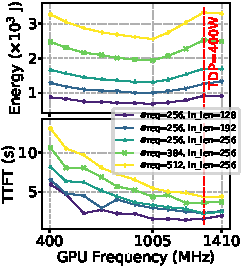
\includegraphics[width=\linewidth]{figs/prefill_energy_ttft.pdf}
    \end{subfigure}
    \hfill
    \begin{subfigure}[b]{0.49\columnwidth}
        \centering
        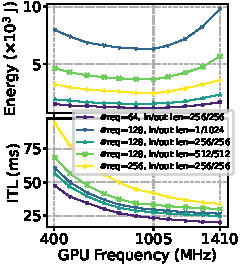
\includegraphics[width=\linewidth]{figs/decode_energy_itl.pdf}
    \end{subfigure}
    \begin{subfigure}[b]{0.49\columnwidth}
        \centering
        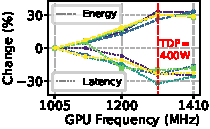
\includegraphics[width=\linewidth]{figs/prefill_energy_latency_diff.pdf}
        \caption{Prefill phase.}
        \label{fig:u-shape-p}
    \end{subfigure}
    \hfill
    \begin{subfigure}[b]{0.49\columnwidth}
        \centering
        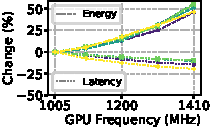
\includegraphics[width=\linewidth]{figs/decode_energy_latency_diff.pdf}
        \caption{Decode phase.}
        \label{fig:u-shape-d}
    \end{subfigure}

    \caption{Impact of GPU frequency on energy (top) and latency (middle) for P/D phases on A100 with LLaMA-3.1-8B.
    The bottom shows the energy and latency relative changes by frequency increases from 1005 MHz to 1410 MHz.
    Prefill hits TDP limitations near 1305 MHz.
    Both phases exhibit U-shaped energy-frequency curves with 1005 MHz as energy-optimal points, but they differ significantly in shape and sensitivity.}
    
    % : prefill is compute-bound and TDP-limited near 1305 MHz, whereas decode is often memory-bound and yields only $\approx$20\% ITL reduction for $\approx$50\% higher energy when increasing frequency from 1005 to 1410 MHz.}
    % These phase-specific trade-offs motivate independent and adaptive frequency control.}
    % \jiahuan{TODO redraw the third row}
    \label{fig:u-shape}
\end{figure}

% \jiahuan{@Minjia, should we move this to the system design section? As it seems too involved}
% The U-shaped curve and P/D phase differences can be explained by two underlying factors.
% First, according to~\cite{gonzalez1997supply}, the dynamic power ($P$) of CMOS circuits, the foundation of GPUs, increases hyper-linearly with frequency ($f$) at high levels due to increased voltage ($V$) (\eref{eq:P-f}).
% Second, the prefill phase is predominantly compute-bound~\cite{agrawal2024taming} and thus benefits continuously from the higher computation capacity at increased frequencies.
% As formalized in \eref{eq:prefill-f}, its execution time is theoretically proportional to $f^{-1}$ and $P^{1/(1+\alpha)}$.
% In contrast, the decode phase is predominantly memory-bound~\cite{agrawal2024taming}.
% Consequently, its performance exhibits sub-linear returns from increased frequency, becoming limited by memory bandwidth rather than computation.
% This relationship is modeled in \eref{eq:decode-f}, where its execution time is proportional to $f^{-(1-\beta)}$ and $P^{(1-\beta)/(1+\alpha)}$.
% \begin{align}
%     P & \propto V^2f \propto f^{1+\alpha}\ (\alpha > 0, \text{when}\ f\ \text{is high}) \label{eq:P-f} \\
%     T_{\text{prefill}} & \propto f^{-1}   \propto P^{\frac{1}{1+\alpha}} \label{eq:prefill-f} \\
%     T_{\text{decode}} & \propto f^{-(1-\beta)}  \propto P^{\frac{1-\beta}{1+\alpha}}\ (0<\beta\le1) \label{eq:decode-f}
% \end{align}




% The differences between P/D phases can be explained by two underlying factors.
% First, for most semiconductors, their power ($P$) increases hyper-linearly with the frequency ($f$) when $f$ is high (\eref{eq:P-f}), due to the increased voltage ($V$)~\cite{vspetko2021dgx}.
% Second, the prefill phase is predominantly compute-bound and therefore can continuously benefit from high frequency.
% As formalized in \eref{eq:prefill-f}, its execution time is proportional to $f^{-1}$ and $P^{1/(1+\alpha)}$ in theory.
% In contrast, the decode phase is predominantly memory-bound.
% Consequently, its performance exhibits sub-linear returns from increased frequency, as execution becomes limited by memory bandwidth rather than computation.
% This relationship is modeled in \eref{eq:decode-f}.
% % , where its execution time is proportional to $f^{-(1-\beta)}$ and $P^{(1-\beta)/(1+\alpha)}$.
% \begin{align}
%     P & \propto V^2f \propto f^{1+\alpha}\ (\alpha > 0, \text{when}\ f\ \text{is high}) \label{eq:P-f} \\
%     T^{\text{prefill}} & \propto f^{-1}   \propto P^{\frac{1}{1+\alpha}}\label{eq:prefill-f} \\
%     T^{\text{decode}} & \propto f^{-(1-\beta)}  \propto P^{\frac{1-\beta}{1+\alpha}}\ (0<\beta\le1)\label{eq:decode-f}
% \end{align}
% This analysis is further supported by \fref{fig:decode-itl-diff}, which illustrates that as the batch size increases, decode phase gradually transits from memory-bound to compute-bound, while the ITL benefits from frequency scaling become larger.
% For LLaMA-3.1-8B served on A100-40G GPU, this turning point is $\sim$150.

% \new{
% The differences between P/D phases can be explained by two underlying factors.

% First, according to \cite{gonzalez1997supply} and \cite{butts2000static}, the dynamic power ($P_{\text{dynamic}}$) of semiconductors increases hyper-linearly with the frequency ($f$) when $f$ is high (\eref{eq:P-f}), due to the increased voltage ($V$)

% }

% \noindent
\textbf{\underline{Insight \#2}}: 
While both P/D phases exhibit U-shaped energy-frequency relationships and the corresponding energy sweet spots, they differ remarkably in shape and sensitivity.
Given that lowering frequency inevitably increases latency, these distinct characteristics motivate an adaptive, phase-aware policy to minimize energy while preserving SLOs. 



% \subsection{Batch Size Boundary-Induced Energy Inefficiency}
\subsection{Architectural Granularity-Induced Energy Inefficiency}
\label{subsec:tile-effect}

% \jiahuan{@Minjia, considering that we change the cause to GEMM tile effect, should we still call it ``Architectural Granularity-Induced Energy Inefficiency''?}
% \minjia{That's still an architecture granularity induced inefficiency, right? }
% \jiahuan{I mean ``architecture'' is more like hardware related, but it can also mean software. If you think it's OK, you can leave it as is.}

% We profile offline serving workloads by varying request numbers for different frequencies.
% As illustrated in \fref{fig:kernel-tile}, while larger batch sizes generally lead to lower EPOT and thus higher energy efficiency, this trend is disrupted at specific thresholds.
% For example, increasing the batch size from 128 to 129 (crossing a "boundary") incurs sudden performance drops, resulting the staircase-like ITL/EPOT relationship to batch size.
% Similar effect exists for the prefill phase, but gets diminished by relatively larger batch token numbers (see Appendix~\ref{appendix:prefill-tile}).

Modern LLM serving systems batch multiple requests to improve GPU utilization~\cite{yu2022orca}.
However, our profiling reveals that implicit batch size boundaries create architecturally induced inefficiencies in both energy and latency, especially during the decode phase.
As shown in \fref{fig:kernel-tile}, while increasing batch sizes generally reduces \textit{Energy-Per-Output-Token} (EPOT) and improves efficiency, this trend is periodically disrupted: crossing certain thresholds (e.g., 256 $\rightarrow$ 257) causes abrupt performance drops, resulting in a ``staircase'' pattern in ITL and EPOT.
A similar but weaker effect exists in prefill, which is masked by its larger token counts (see \appref{appendix:prefill-tile}).


% This phenomenon can be attributed to hardware under-utilization known as the GPU tail effect~\cite{yu2020towards}.
% A GPU processes large workloads by breaking them into sequential ``waves'' of thread blocks that run for a fixed processing cycle.
% When the last wave of a workload cannot fully occupy the GPU's Streaming Multiprocessors (SMs), the hardware is under-utilized.
% However, this partially filled wave still consumes a full processing cycle, leading to a disproportionate increase in latency and creating a ``latency staircase'' pattern rather than a smooth, linear improvement.
% In coupled architectures that handle prefill and decode on the same GPU, techniques like chunked prefill~\cite{agrawal2024taming} can mitigate this issue by mixing prefill and decode tokens into same batches. 
% However, in a P/D disaggregated architecture, the small number of batched tokens in the decode instance makes it an unignorable problem.
% This is a critical inefficiency that is overlooked by popular LLM serving frameworks like SGLang and vLLM.

% This discontinuities arise from SM-level tiling and scheduling granularity within GPU kernel execution.
% Large batches are decomposed into multiple ``waves'' of thread blocks scheduled across Streaming Multiprocessors (SMs).
% When the final wave cannot fully occupy all SMs, the GPU executes a partially filled cycle that consumes full power but delivers lower throughput, which creates visible steps in energy and latency in \fref{fig:kernel-tile}.
% This is similar to the tail effect~\cite{yu2020towards}, but here it manifests as an energy-latency ``staircase'' due to decode workload's small batch sizes.
% \junfeng{

This discontinuity arises from tile quantization.
GPUs execute GEMM by partitioning the output matrix into fixed-size ``tiles'' and assigning them to thread blocks~\cite{gemmtile}.
This ``staircase'' effect occurs when the batch size is not an exact multiple of the tile dimensions.
For example, as \fref{fig:gemm-tile} shows, when the batch size increases from 256 to 257, the GPU must launch an entirely new, but almost empty, tile (e.g., only 6.25\% useful data) to process this single extra request. 
This under-utilized tile requires the same execution time (duration) as a fully utilized tile. This leads to an increase in the total number of tiles, which in turn causes a sudden jump in latency (ITL) and a drop in efficiency (EPOT), forming the ``staircase’’ seen in \fref{fig:kernel-tile}.
While coupled serving architectures (e.g., chunked prefill~\cite{agrawal2024taming}) can mask this behavior by merging prefill and decode tokens into shared kernels, P/D disaggregated architecture amplifies the problem, as the decode instances operate with smaller, highly variable batch sizes. 

\begin{figure}[t]
    \centering
    \begin{minipage}[b]{0.49\columnwidth}
        \centering
        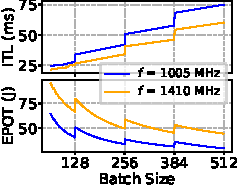
\includegraphics[width=\linewidth]{figs/energy_tile.pdf}
        \caption{Batch size boundary and ``staircase'' effects in ITL and EPOT in the decode phase.}
        \label{fig:kernel-tile}
    \end{minipage}
    \hfill
    \begin{minipage}[b]{0.49\columnwidth}
        \centering
        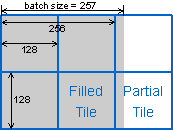
\includegraphics[width=\columnwidth]{figs/voltanallm-gemm-tile.drawio.pdf}
        \caption{The tile quantization effect of GEMM. Tile size is 128, and request batch size is 257.}
        \label{fig:gemm-tile}
    \end{minipage}
\end{figure}

\textbf{\underline{Insight \#3}}: GPU architectural granularity, specifically SM-level tiling and scheduling boundaries, causes discontinuous ``staircase'' effects in energy and latency as batch sizes cross certain thresholds.
This hardware-level phenomenon is amplified in P/D disaggregated LLM inference, and reveals an overlooked source of energy inefficiency and motivates architecture-aware frequency and batching control.